\chapter{表面、吸附与多相催化}\label{ch:b3:surfaces-catalysis}

汽车底部的钢罐内装有一块陶瓷蜂窝体，其成千上万条
孔道上涂有多孔氧化物，负载着几克铂、
钯和铑。在不到一秒的时间内，流经其中的废气
便失去了大部分一氧化碳、未燃烬的烃类和
氮氧化物。气相中并不发生任何变化：这些反应
都发生在直径仅几纳米的金属颗粒表面。化学工业的大部分
过程也是如此，从化肥用氨到石油裂解。
本章讨论分子如何附着于表面、表面被覆盖的程度，
表面反应如何进行，以及固体催化剂如何
制备、测量和观察。

\begin{recall}
本科一年级分册定义了催化剂，以及均相催化与
多相催化的区别，并描述了金属的面心立方堆积。
本科二年级分册定义了催化剂的转化率、选择性和
转化频率，并介绍了勒夏特列原理。
\Cref{ch:b3:x-ray-diffraction}介绍了\omterm{def:b3:x-ray-diffraction:miller}{米勒指数}，
\cref{ch:b3:rate-theories}介绍了\omterm{thm:b3:rate-theories:eyring}{艾林方程}，
\cref{ch:b3:partition-functions}介绍了分布的统计。
\end{recall}

\begin{omfigure}
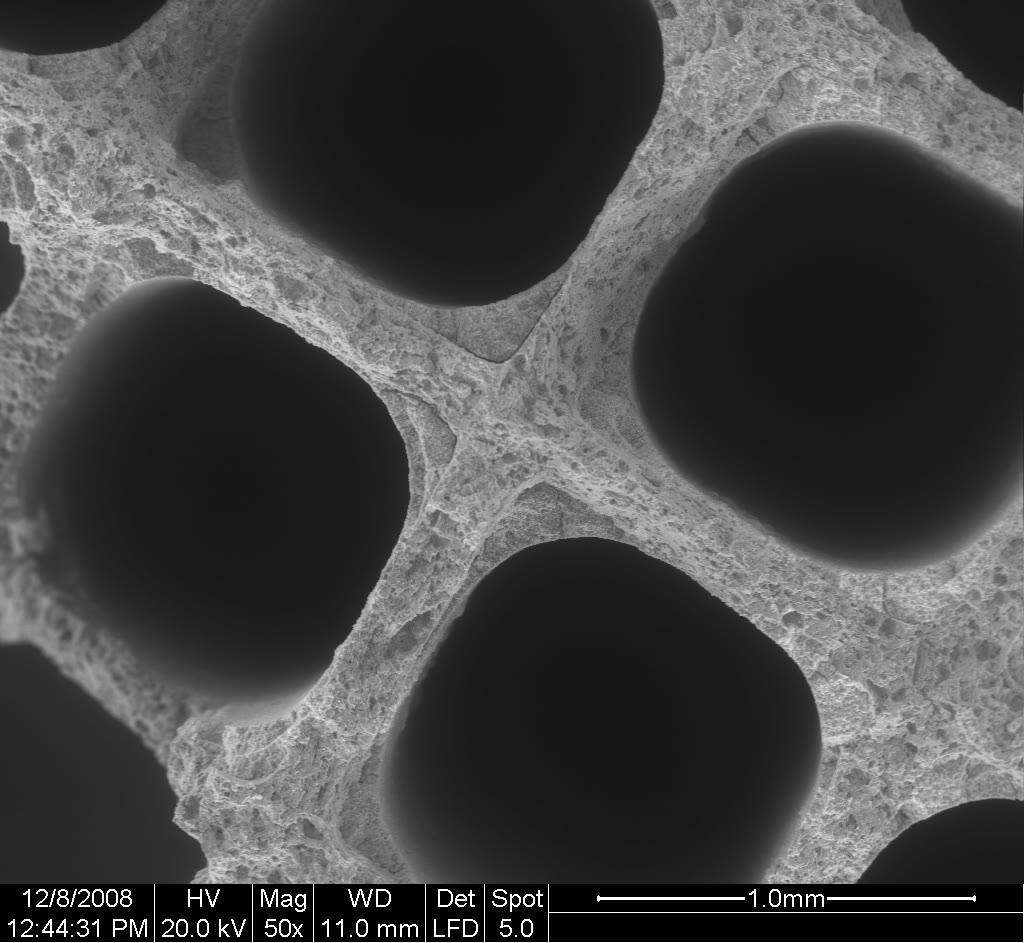
\includegraphics[width=0.48\linewidth]{images/book4/converter-sem.jpg}

{\small 催化转化器的陶瓷蜂窝体经扫描
电子显微镜观察（标尺 \qty{1.0}{mm}）：方形孔道由薄的
多孔壁隔开，孔壁上负载着氧化物涂层及其中的金属颗粒。}
\end{omfigure}

\section{吸附}

\begin{definition}[吸附]\label{def:b3:surfaces-catalysis:adsorption}
\emph{吸附}\index{吸附}是气体或溶质的分子在
固体或液体表面聚集的过程。发生吸附的分子称为
\emph{吸附质}\index{吸附质}，固体称为\emph{吸附剂}\index{吸附剂}；
其逆过程称为\emph{脱附}\index{脱附}。
\end{definition}

\begin{definition}[物理吸附、化学吸附]\label{def:b3:surfaces-catalysis:physi-chemi}
\emph{物理吸附}\index{物理吸附}是由范德瓦耳斯力引起的\omterm{def:b3:surfaces-catalysis:adsorption}{吸附}，
\omterm{def:b3:surfaces-catalysis:adsorption}{吸附}焓至多为几十千焦每摩尔，
与凝结焓相当，分子本身不发生变化。
\emph{化学吸附}\index{化学吸附}与表面形成化学键，
\omterm{def:b3:surfaces-catalysis:adsorption}{吸附}焓约为 40 至几百千焦每摩尔；它可以
使分子解离（解离化学\omterm{def:b3:surfaces-catalysis:adsorption}{吸附}），且只能形成单层。
\end{definition}

\begin{omfigure}
\begin{tikzpicture}[font=\small, >=Stealth, x=1cm, y=1cm]
  \draw[->] (0,-2.6) -- (0,1.8) node[anchor=south] {能量};
  \draw[->] (0,0) -- (8.0,0) node[anchor=south east] {距表面的距离};
  \draw[omDef, thick] plot[smooth, tension=0.7] coordinates {(1.6,1.6) (2.2,-0.25) (2.8,-0.62) (3.6,-0.35) (5.0,-0.08) (7.5,0)};
  \draw[omThm, thick] plot[smooth, tension=0.6] coordinates {(0.45,1.6) (0.8,-1.2) (1.2,-2.2) (1.7,-1.6) (2.35,-0.15) (2.9,0.9) (3.5,1.5)};
  \node[omDef, anchor=north west, font=\scriptsize] at (3.4,-0.4) {物理吸附的 \ce{H2}（前驱态）};
  \node[omThm, anchor=west, font=\scriptsize] at (1.75,-1.9) {化学吸附的 2 H};
  \node[omThm, anchor=west, font=\scriptsize, align=left] at (3.55,1.45) {趋向 $\mathrm{H} + \mathrm{H}$\\ 远离表面};
  \fill (2.3,-0.2) circle (1.5pt);
  \node[font=\scriptsize] (cr) at (1.25,0.55) {交叉点};
  \draw[black!60] (cr.south east) -- (2.27,-0.15);
\end{tikzpicture}

{\small 氢分子接近金属表面时的势能（示意）。
分子先落入较浅的\omterm{def:b3:surfaces-catalysis:physi-chemi}{物理吸附}势阱；
在此曲线与两个各自成键的 H 原子曲线相交处，它可以
解离进入较深的\omterm{def:b3:surfaces-catalysis:physi-chemi}{化学吸附}势阱。若交叉点位于零能级之上，
则解离\omterm{def:b3:surfaces-catalysis:physi-chemi}{化学吸附}需要活化。}
\end{omfigure}

金属颗粒的表面主要暴露面心立方晶格中最密排的
\omterm{def:b3:x-ray-diffraction:miller}{晶面}，即 (111) 面和 (100) 面。在这些表面上，\omterm{def:b3:surfaces-catalysis:adsorption}{吸附质}可以位于一个原子之上
（顶位）、两个原子之间（桥位），或位于三个或四个原子形成的空穴中，并且
不同位置的结合能各不相同。

\begin{omfigure}
\begin{tikzpicture}[font=\scriptsize]
  % fcc(111): hexagonal layer, spacing 0.6 cm
  \foreach \i in {0,...,5}{\foreach \j in {0,...,4}{
    \shade[ball color=black!25] ({0.6*\i+0.3*\j},{0.52*\j}) circle (0.29);}}
  \fill[omThm] (1.2+0.3*1,0.52) circle (0.07);
  \fill[omDef] ({0.6*2+0.3*2+0.3},{0.52*2}) circle (0.07);
  \fill[black] ({0.6*3+0.3*2+0.3},{0.52*2+0.17}) circle (0.07);
  \fill[black!60!green] ({0.6*1+0.3*3+0.3},{0.52*3-0.17}) circle (0.07);
  \node[anchor=north] at (2.1,-0.45) {面心立方 (111)};
  % fcc(100): square layer
  \begin{scope}[xshift=5.6cm]
  \foreach \i in {0,...,4}{\foreach \j in {0,...,4}{
    \shade[ball color=black!25] ({0.6*\i},{0.6*\j}) circle (0.29);}}
  \fill[omThm] (1.2,1.2) circle (0.07);
  \fill[omDef] (1.5,1.8) circle (0.07);
  \fill[black] (2.1,0.9) circle (0.07);
  \node[anchor=north] at (1.2,-0.45) {面心立方 (100)};
  \end{scope}
  \node[anchor=west, align=left] at (9.0,1.6) {\textcolor{omThm}{$\bullet$} 顶位 \\ \textcolor{omDef}{$\bullet$} 桥位 \\
    $\bullet$ 空穴（三重或四重）\\ \textcolor{black!60!green}{$\bullet$} 第二类三重空穴 (111)};
\end{tikzpicture}

{\small 面心立方金属两个最密排\omterm{def:b3:x-ray-diffraction:miller}{晶面}的俯视图，并标出\omterm{def:b3:surfaces-catalysis:adsorption}{吸附}位：
顶位为一个原子之上，桥位为两个原子之间，并位于
(111) 面上三个原子之间的空穴（分两类：位于第二层原子之上或不在其上），或
(100) 面上四个原子之间的空穴。}
\end{omfigure}

\begin{definition}[覆盖度、单分子层]\label{def:b3:surfaces-catalysis:coverage}
表面的\emph{覆盖度}\index{覆盖度} $\theta$ 是其被占据的
\omterm{def:b3:surfaces-catalysis:adsorption}{吸附}位数占全部\omterm{def:b3:surfaces-catalysis:adsorption}{吸附}位数的分数。
\emph{单分子层}\index{单分子层}是\omterm{def:b3:surfaces-catalysis:adsorption}{吸附质}形成的单一完整层，此时 $\theta = 1$。
\end{definition}

\section{等温线}

\begin{theorem}[朗缪尔等温式]\label{thm:b3:surfaces-catalysis:langmuir}
若表面具有相同且彼此独立的\omterm{def:b3:surfaces-catalysis:adsorption}{吸附}位，每个\omterm{def:b3:surfaces-catalysis:adsorption}{吸附}位仅容纳一个分子，则
与压强为 $p$ 的气体达到平衡时，\omterm{def:b3:surfaces-catalysis:coverage}{覆盖度}为
\[
  \theta = \frac{Kp}{1 + Kp},
\]
其中 $K$ 为\omterm{def:b3:surfaces-catalysis:adsorption}{吸附}平衡常数，仅依赖于
温度。此式即\emph{朗缪尔等温式}\index{朗缪尔等温式}。
\end{theorem}

\begin{proof}
动力学证明。分子在空闲\omterm{def:b3:surfaces-catalysis:adsorption}{吸附}位上的\omterm{def:b3:surfaces-catalysis:adsorption}{吸附}速率为 $k_ap(1 - \theta)N$（$N$
\omterm{def:b3:surfaces-catalysis:adsorption}{吸附}位数），\omterm{def:b3:surfaces-catalysis:adsorption}{脱附}速率为 $k_d\theta N$。平衡时两者相等：$\theta/(1 - \theta)
= (k_a/k_d)p$，整理即得结论，其中 $K = k_a/k_d$。

统计证明。$M$ 个分子占据 $N$ 个\omterm{def:b3:surfaces-catalysis:adsorption}{吸附}位，共有 $N!/(M!(N - M)!)$ 种排布方式，
每个被\omterm{def:b3:surfaces-catalysis:adsorption}{吸附}分子具有内部配分函数 $q_{\mathrm s}$（其
与表面之间的振动及其结合能）。由斯特林公式
可得\omterm{def:b3:surfaces-catalysis:adsorption}{吸附}分子的化学势为 $\mu_{\mathrm s} = -kT\ln\bigl(q_{\mathrm s}\frac{1 - \theta}{\theta}\bigr)$；
理想气体的为 $\mu_{\mathrm g} = \mu_{\mathrm g}^\circ + kT\ln(p/p^\circ)$。平衡时 $\mu_{\mathrm s} = \mu_{\mathrm g}$，得
$\theta/(1 - \theta) = q_{\mathrm s}\eu^{\mu_{\mathrm g}^\circ/kT}p/p^\circ$：与上式形式相同，只是 $K$ 用
配分函数表示。
\end{proof}

低压时 $\theta \approx Kp$（亨利区）；高压时 $\theta \to 1$。
压强为 $p = 1/K$ 时，\omterm{def:b3:surfaces-catalysis:coverage}{覆盖度}恰为一半。

\begin{proposition}[解离吸附]\label{prop:b3:surfaces-catalysis:dissociative}
对于在两个\omterm{def:b3:surfaces-catalysis:adsorption}{吸附}位上解离的双原子气体，$\mathrm{H_2} + 2\,{*} \to 2\,\mathrm{H}{*}$（${*}$：空闲\omterm{def:b3:surfaces-catalysis:adsorption}{吸附}位），
\[
  \theta = \frac{(Kp)^{1/2}}{1 + (Kp)^{1/2}},
\]
因此低压时 $\theta \propto \sqrt p$。
\end{proposition}

\begin{proof}
\omterm{def:b3:surfaces-catalysis:adsorption}{吸附}需要两个空闲\omterm{def:b3:surfaces-catalysis:adsorption}{吸附}位，速率为 $k_ap(1 - \theta)^2$；\omterm{def:b3:surfaces-catalysis:adsorption}{脱附}需要两个被\omterm{def:b3:surfaces-catalysis:adsorption}{吸附}的
原子复合，速率为 $k_d\theta^2$。由平衡条件得 $\theta/(1 - \theta) =
(Kp)^{1/2}$。
\end{proof}

\begin{proposition}[竞争吸附]\label{prop:b3:surfaces-catalysis:competitive}
两种气体 A 和 B 争夺同一\omterm{def:b3:surfaces-catalysis:adsorption}{吸附}位，它们的\omterm{def:b3:surfaces-catalysis:coverage}{覆盖度}分别为
\[
  \theta_{\mathrm A} = \frac{K_{\mathrm A}p_{\mathrm A}}{1 + K_{\mathrm A}p_{\mathrm A} + K_{\mathrm B}p_{\mathrm B}}, \qquad
  \theta_{\mathrm B} = \frac{K_{\mathrm B}p_{\mathrm B}}{1 + K_{\mathrm A}p_{\mathrm A} + K_{\mathrm B}p_{\mathrm B}} .
\]
\end{proposition}

\begin{proof}
对每种气体，$k_{a,\mathrm A}p_{\mathrm A}(1 - \theta_{\mathrm A} - \theta_{\mathrm B}) = k_{d,\mathrm A}\theta_{\mathrm A}$，对 B 同理。于是
$\theta_{\mathrm A} = K_{\mathrm A}p_{\mathrm A}\theta_\ast$，$\theta_{\mathrm B} = K_{\mathrm B}p_{\mathrm B}\theta_\ast$，其中 $\theta_\ast = 1 - \theta_{\mathrm A} - \theta_{\mathrm B}$ 为空闲分数；两式相加，
$1 - \theta_\ast = \theta_\ast(K_{\mathrm A}p_{\mathrm A} + K_{\mathrm B}p_{\mathrm B})$。
\end{proof}

\begin{definition}[等量吸附焓]\label{def:b3:surfaces-catalysis:isosteric}
\emph{等量吸附焓}\index{等量吸附焓}
$\Delta_{\mathrm{ads}}H$ 是在固定\omterm{def:b3:surfaces-catalysis:coverage}{覆盖度}下的摩尔\omterm{def:b3:surfaces-catalysis:adsorption}{吸附}焓，
由在不同温度下给出相同\omterm{def:b3:surfaces-catalysis:coverage}{覆盖度}的压强
求得。
\end{definition}

\begin{proposition}[等量吸附焓]\label{prop:b3:surfaces-catalysis:isosteric}
在\omterm{def:b3:surfaces-catalysis:coverage}{覆盖度}恒定时，
\[
  \Bigl(\frac{\partial\ln p}{\partial T}\Bigr)_\theta = -\frac{\Delta_{\mathrm{ads}}H}{RT^2} .
\]
\end{proposition}

\begin{proof}
\omterm{def:b3:surfaces-catalysis:coverage}{覆盖度} $\theta$ 恒定时，$Kp$ 为常数（对于朗缪尔表面；一般情形下，同样的
论证对该\omterm{def:b3:surfaces-catalysis:coverage}{覆盖度}下的平衡常数同样成立），故 $\ln p =
\text{常数} - \ln K$。由范托夫方程，$\dd\ln K/\dd T = \Delta_{\mathrm{ads}}H/RT^2$（$K$
参照标准压强）。
\end{proof}

由于\omterm{def:b3:surfaces-catalysis:adsorption}{吸附}为放热过程，温度升高时，要达到相同\omterm{def:b3:surfaces-catalysis:coverage}{覆盖度}需要更高的压强：
图中等温线随 $T$ 升高而下降。

\begin{theorem}[BET 等温式]\label{thm:b3:surfaces-catalysis:bet}
若分子逐层\omterm{def:b3:surfaces-catalysis:adsorption}{吸附}，第一层具有表面特有的结合常数，
其余各层则具有液体的凝结平衡，
则在相对压强 $x = p/p^*$（$p^*$：液态\omterm{def:b3:surfaces-catalysis:adsorption}{吸附质}的蒸气
压）下的\omterm{def:b3:surfaces-catalysis:adsorption}{吸附}量为
\[
  \frac{v}{v_{\mathrm m}} = \frac{cx}{(1 - x)(1 - x + cx)},
\]
其中 $v_{\mathrm m}$ 为\omterm{def:b3:surfaces-catalysis:coverage}{单分子层}中的\omterm{def:b3:surfaces-catalysis:adsorption}{吸附}量，$c$ 为与第一层\omterm{def:b3:surfaces-catalysis:adsorption}{吸附}焓
和凝结焓之差有关的常数。此式即
\emph{BET 等温式}\index{BET 等温式}（布鲁诺尔、
埃米特和泰勒）。
\end{theorem}

\begin{proof}
设 $s_i$ 为恰被 $i$ 层覆盖的表面分数。
对每一层作平衡（与朗缪尔证明中相同），得 $s_1 = cxs_0$，且 $s_i =
xs_{i-1}$（$i \ge 2$），故 $s_i = cx^is_0$。被\omterm{def:b3:surfaces-catalysis:adsorption}{吸附}量为 $v/v_{\mathrm m} =
\sum_iis_i/\sum_is_i$。利用 $\sum_{i\ge1}x^i = x/(1 - x)$ 与 $\sum_{i\ge1}ix^i = x/(1 - x)^2$，得：
\[
  \frac{v}{v_{\mathrm m}} = \frac{cs_0\,x/(1 - x)^2}{s_0[1 + cx/(1 - x)]} = \frac{cx}{(1 - x)(1 - x + cx)} .
\]
\end{proof}

整理得 $\dfrac{x}{v(1 - x)} = \dfrac{1}{v_{\mathrm m}c} + \dfrac{c - 1}{v_{\mathrm m}c}\,x$，这是一条直线，其斜率与
截距分别给出 $v_{\mathrm m}$ 与 $c$，通常适用于 $0.05 < x < 0.30$ 的范围。

\begin{definition}[比表面积]\label{def:b3:surfaces-catalysis:surface-area}
固体的\emph{比表面积}\index{比表面积}是其
单位质量的表面积，包括孔道内壁。
\end{definition}

\begin{method}[由氮气等温线测定比表面积]\label{met:b3:surfaces-catalysis:bet-area}
\begin{enumerate}
  \item 在真空下一边加热一边对样品脱气；随后用液氮冷却
        (\qty{77}{K}).
  \item 测量\omterm{def:b3:surfaces-catalysis:adsorption}{吸附}的氮气体积（换算为标准状况），
        相对压强在 0.05 至 0.30 之间。
  \item 以 $x/(v(1 - x))$ 对 $x$ 作图；由斜率与截距，
        则 $v_{\mathrm m} = 1/(\text{斜率} + \text{截距})$，$c = 1 + \text{斜率}/\text{截距}$。
  \item 面积 $= n_{\mathrm m}N_Aa_{\mathrm m}$，其中 $n_{\mathrm m}$ 为\omterm{def:b3:surfaces-catalysis:coverage}{单分子层}中的物质的量，$a_{\mathrm m} = \qty{0.162}{nm^2}$
        为一个被\omterm{def:b3:surfaces-catalysis:adsorption}{吸附}氮分子的常用面积。
\end{enumerate}
\end{method}

\begin{omfigure}
\begin{tikzpicture}
\begin{axis}[name=la, width=0.31\linewidth, height=5.0cm, xmin=0, xmax=100, ymin=0, ymax=1.05,
  axis lines=left, xlabel={压强 $p$ / 千帕}, ylabel={$\theta$}, tick label style={font=\small},
  label style={font=\small}, title={\small 朗缪尔}]
\addplot[omDef, thick] table[x=p_kPa, y=T300] {figdata/out/bachelor-3-langmuir-bet-langmuir.dat};
\addplot[omThm, thick] table[x=p_kPa, y=T350] {figdata/out/bachelor-3-langmuir-bet-langmuir.dat};
\node[font=\scriptsize, omDef, anchor=south east] at (axis cs:98,0.92) {\qty{300}{K}};
\node[font=\scriptsize, omThm, anchor=north east] at (axis cs:98,0.45) {\qty{350}{K}};
\end{axis}
\begin{axis}[name=be, at={(la.east)}, anchor=west, xshift=1.9cm, width=0.31\linewidth, height=5.0cm,
  xmin=0, xmax=0.9, ymin=0, ymax=200, axis lines=left, xlabel={$p/p^*$},
  ylabel={$v$ / \unit{cm^3.g^{-1}}}, tick label style={font=\small}, label style={font=\small},
  title={\small BET 等温式}]
\addplot[black, thick] table[x=x, y=v] {figdata/out/bachelor-3-langmuir-bet-bet.dat};
\addplot[only marks, mark=*, mark size=1.4pt, omDef] table[x=x, y=v] {figdata/out/bachelor-3-langmuir-bet-data.dat};
\draw[black!40, dashed] (axis cs:0,45) -- (axis cs:0.9,45);
\node[font=\scriptsize, anchor=south east] at (axis cs:0.88,45) {$v_{\mathrm m}$};
\end{axis}
\begin{axis}[at={(be.east)}, anchor=west, xshift=2.1cm, width=0.31\linewidth, height=5.0cm,
  xmin=0, xmax=0.35, ymin=0, ymax=0.0085, axis lines=left, xlabel={$x = p/p^*$},
  ylabel={$x/(v(1 - x))$}, tick label style={font=\small}, label style={font=\small},
  scaled y ticks=false, yticklabel style={/pgf/number format/fixed, /pgf/number format/precision=3},
  title={\small BET 线性图}]
\addplot[black, thin] table[x=x, y=y] {figdata/out/bachelor-3-langmuir-bet-line.dat};
\addplot[only marks, mark=*, mark size=1.4pt, omDef] table[x=x, y=y] {figdata/out/bachelor-3-langmuir-bet-data.dat};
\end{axis}
\end{tikzpicture}

{\small 左：模型\omterm{def:b3:surfaces-catalysis:physi-chemi}{化学吸附}（$\Delta_{\mathrm{ads}}H = \qty{-40}{kJ/mol}$）在两个温度下的\omterm{thm:b3:surfaces-catalysis:langmuir}{朗缪尔等温式}。中：
BET 等温式（模型，$v_{\mathrm m} = \qty{45}{cm^3.g^{-1}}$，$c = 120$），并标出
周末问题中的数据点；\omterm{def:b3:surfaces-catalysis:adsorption}{吸附}层不断堆积，\omterm{def:b3:surfaces-catalysis:adsorption}{吸附}量在
$p = p^*$ 附近发散，此处气体凝结。右：同一组数据点的 BET 线性图。}
\end{omfigure}

\section{表面反应动力学}

\begin{definition}[朗缪尔–欣谢尔伍德机理与埃利–里迪尔机理]\label{def:b3:surfaces-catalysis:mechanisms}
在\emph{朗缪尔–欣谢尔伍德机理}\index{朗缪尔–欣谢尔伍德机理}中，
两种反应物均\omterm{def:b3:surfaces-catalysis:adsorption}{吸附}在表面并在表面上反应；在
\emph{埃利–里迪尔机理}\index{埃利–里迪尔机理}中，\omterm{def:b3:surfaces-catalysis:adsorption}{吸附}的反应物
与来自气相的分子发生反应。
\end{definition}

\begin{proposition}[朗缪尔–欣谢尔伍德速率]\label{prop:b3:surfaces-catalysis:lh-rate}
若\omterm{def:b3:surfaces-catalysis:adsorption}{吸附}平衡迅速建立，且\omterm{def:b3:surfaces-catalysis:adsorption}{吸附}态 A 与 B 之间的表面反应
为决速步，则
\[
  r = k\theta_{\mathrm A}\theta_{\mathrm B} = \frac{kK_{\mathrm A}p_{\mathrm A}K_{\mathrm B}p_{\mathrm B}}{(1 + K_{\mathrm A}p_{\mathrm A} + K_{\mathrm B}p_{\mathrm B})^2},
\]
在 $p_{\mathrm B}$ 固定时，速率在 $K_{\mathrm A}p_{\mathrm A} = 1 + K_{\mathrm B}p_{\mathrm B}$ 时最大，此后随着 A 将 B 挤出
表面而下降。
\end{proposition}

\begin{proof}
\omterm{def:b3:surfaces-catalysis:coverage}{覆盖度}由\cref{prop:b3:surfaces-catalysis:competitive}给出。令 $u =
K_{\mathrm A}p_{\mathrm A}$，$a = 1 + K_{\mathrm B}p_{\mathrm B}$，则 $r \propto u/(a + u)^2$，其导数 $(a - u)/(a + u)^3$ 在
$u = a$ 处为零。
\end{proof}

\begin{proposition}[埃利–里迪尔速率]\label{prop:b3:surfaces-catalysis:er-rate}
若\omterm{def:b3:surfaces-catalysis:adsorption}{吸附}的 A 与气态 B 反应，则
\[
  r = k\theta_{\mathrm A}p_{\mathrm B} = \frac{kK_{\mathrm A}p_{\mathrm A}p_{\mathrm B}}{1 + K_{\mathrm A}p_{\mathrm A}},
\]
速率随 $p_{\mathrm A}$ 增大并趋于平台，不存在极大值。
\end{proposition}

\begin{proof}
B 不与 A 竞争\omterm{def:b3:surfaces-catalysis:adsorption}{吸附}位点：$\theta_{\mathrm A}$ 即仅由 A 决定的朗缪尔\omterm{def:b3:surfaces-catalysis:coverage}{覆盖度}，且
速率正比于它以及 B 与表面的碰撞速率，
后者正比于 $p_{\mathrm B}$。
\end{proof}

\begin{method}[由压强依赖关系判断为 LH 还是 ER]\label{met:b3:surfaces-catalysis:mechanism-from-rate}
\begin{enumerate}
  \item 逐一测量速率随每种反应物压强的变化，另一反应物的压强保持
        不变。
  \item 出现极大值，随后下降（高压下为负级数）：
        \omterm{def:b3:surfaces-catalysis:mechanisms}{朗缪尔–欣谢尔伍德机理}，反应物因占据位点而起抑制作用。
  \item 某一反应物的速率上升至平台，而另一反应物在各压强下均为一级：
        \omterm{def:b3:surfaces-catalysis:mechanisms}{埃利–里迪尔机理}。
  \item 用同位素标记或表面谱学加以确认；多数催化
        反应属于朗缪尔–欣谢尔伍德类型。
\end{enumerate}
\end{method}

\begin{omfigure}
\begin{tikzpicture}
\begin{axis}[width=0.6\linewidth, height=5.4cm, xmin=0, xmax=10, ymin=0, ymax=0.3,
  axis lines=left, xlabel={$p_{\mathrm A}$（约化）}, ylabel={速率（约化）},
  tick label style={font=\small}, label style={font=\small},
  legend style={font=\scriptsize, draw=none, at={(1.03,0.98)}, anchor=north west}, legend cell align=left]
\addplot[omDef!50, thick] table[x=pA, y=pB05] {figdata/out/bachelor-3-surface-rates.dat};
\addplot[omDef, thick] table[x=pA, y=pB1] {figdata/out/bachelor-3-surface-rates.dat};
\addplot[black, thick] table[x=pA, y=pB3] {figdata/out/bachelor-3-surface-rates.dat};
\addplot[omThm, thick, dashed] table[x=pA, y=ER] {figdata/out/bachelor-3-surface-rates.dat};
\legend{{LH，$p_{\mathrm B} = 0.5$}, {LH，$p_{\mathrm B} = 1$}, {LH，$p_{\mathrm B} = 3$}, {ER（$\times\frac14$）}}
\end{axis}
\end{tikzpicture}

{\small 双分子表面反应的速率随 A 的压强变化
（约化单位，$K_{\mathrm A} = K_{\mathrm B} = 1$）。\omterm{def:b3:surfaces-catalysis:mechanisms}{朗缪尔–欣谢尔伍德机理}：每条曲线在 $K_{\mathrm A}p_{\mathrm A} =
1 + K_{\mathrm B}p_{\mathrm B}$ 处达到峰值，随后随 A 取代 B 而下降。\omterm{def:b3:surfaces-catalysis:mechanisms}{埃利–里迪尔机理}（虚线，经缩放）：呈平台。}
\end{omfigure}

\begin{proposition}[表观活化能]\label{prop:b3:surfaces-catalysis:apparent-ea}
对于伴有朗缪尔\omterm{def:b3:surfaces-catalysis:adsorption}{吸附}的单分子表面反应，$r = k\theta = kKp/(1 + Kp)$。
在低\omterm{def:b3:surfaces-catalysis:coverage}{覆盖度}下，测得的活化能为 $E_{a,\mathrm{app}} = E_a + \Delta_{\mathrm{ads}}H$；在
高\omterm{def:b3:surfaces-catalysis:coverage}{覆盖度}下则为 $E_a$。
\end{proposition}

\begin{proof}
低\omterm{def:b3:surfaces-catalysis:coverage}{覆盖度}下 $r \approx kKp$，故 $\dd\ln r/\dd T = \dd\ln k/\dd T + \dd\ln K/\dd T = (E_a + \Delta_{\mathrm{ads}}H)/RT^2$。
高\omterm{def:b3:surfaces-catalysis:coverage}{覆盖度}下 $\theta \approx 1$，$r \approx k$。
\end{proof}

由于 $\Delta_{\mathrm{ads}}H < 0$，稀疏覆盖表面上的反应看起来比其
真实能垒低：升高温度加快了表面步骤，却也使表面
趋于空出。

\begin{definition}[萨巴蒂尔原理、火山图]\label{def:b3:surfaces-catalysis:sabatier}
\emph{萨巴蒂尔原理}\index{萨巴蒂尔原理}指出，最佳
催化剂对反应物的结合既不宜过弱（反应物不\omterm{def:b3:surfaces-catalysis:adsorption}{吸附}或
不被活化），也不宜过强（产物不脱离而堵塞位点）。
\emph{火山图}\index{火山图}描述一系列催化剂的活性
随结合能的变化，在结合适中时取最大值。
\end{definition}

\begin{omfigure}
\begin{tikzpicture}[font=\small, >=Stealth]
  \draw[->] (0,0) -- (7.2,0) node[anchor=north east] {吸附质的结合强度};
  \draw[->] (0,0) -- (0,3.6) node[anchor=south] {活性};
  \draw[omDef, very thick] (0.4,0.3) -- (3.4,3.0) -- (6.6,0.4);
  \node[anchor=south, align=center, font=\scriptsize] at (1.35,2.0) {结合过弱：\\ 反应物未 \\ 被活化};
  \node[anchor=south, align=center, font=\scriptsize] at (5.9,2.0) {结合过强：\\ 产物堵塞 \\ 活性位点};
  \node[anchor=south, font=\scriptsize] at (3.4,3.05) {最佳催化剂};
\end{tikzpicture}

{\small \omterm{def:b3:surfaces-catalysis:sabatier}{火山图}（定性示意）：一系列催化剂的活性
随其结合关键中间体的强度而变化。}
\end{omfigure}

\section{工业催化剂}

\begin{definition}[催化剂设计]\label{def:b3:surfaces-catalysis:catalyst-design}
\emph{催化剂载体}\index{催化剂载体}是一种多孔、高\omterm{def:b3:surfaces-catalysis:surface-area}{比表面积}的固体
（氧化铝、二氧化硅、碳），其上负载着活性相的小颗粒。
\emph{助催化剂}\index{助催化剂}是一种单独无活性、但能提高
活性、选择性或稳定性的添加剂。\emph{催化剂毒物}\index{催化剂毒物}
是一种与\omterm{def:b3:complex-kinetics:enzyme}{活性位点}强烈结合并将其堵塞的物质。
\emph{金属分散度}\index{金属分散度} $D$ 是位于表面的
金属原子所占的分数。\emph{烧结}\index{烧结}是指高温下颗粒长大，
从而使分散度降低。
\end{definition}

\begin{method}[由氢化学吸附求分散度与粒径]\label{met:b3:surfaces-catalysis:dispersion}
\begin{enumerate}
  \item 在氢气中还原催化剂，抽真空，测量金属上\omterm{def:b3:surfaces-catalysis:physi-chemi}{化学吸附}的 \ce{H2}
        体积（换算为标准状况）；
        载体对此无\omterm{def:b3:surfaces-catalysis:adsorption}{吸附}。
  \item 假设每个表面金属原子对应一个 H 原子：$D = n_{\ce{H}}/n_{\text{金属}}$。
  \item 对直径为 $d$ 的球形颗粒，$D = 6(v_{\mathrm{at}}/a_{\mathrm{at}})/d$，其中 $v_{\mathrm{at}}$ 为块体中每个原子的体积，
        $a_{\mathrm{at}}$ 为每个表面原子所占的面积；由此得 $d = 6v_{\mathrm{at}}/(a_{\mathrm{at}}D)$。
\end{enumerate}
\end{method}

合成氨反应 $\ce{N2 + 3 H2 <=> 2 NH3}$ 约在 400 至 \qty{500}{\celsius}、100 至
\qty{300}{bar} 下进行，催化剂为添加了氧化钾和氧化铝的铁：
氧化铝防止铁微晶\omterm{def:b3:surfaces-catalysis:catalyst-design}{烧结}，钾则提高活性。
决速步是 \ce{N2} 的解离\omterm{def:b3:surfaces-catalysis:physi-chemi}{化学吸附}，其
三键是最难断开的化学键。全世界每年约
有 1.5 亿吨氮以此方式被固定。
% ledger: nh3:world-2024
在以硫酸钾为\omterm{def:b3:surfaces-catalysis:catalyst-design}{助催化剂}的五氧化二钒上，\ce{SO2} 氧化为 \ce{SO3}，
是硫酸生产中的关键一步。

汽油机的三效催化转化器能氧化 CO 和碳氢化合物，
同时还原氮氧化物。所用金属为铂和钯（起氧化作用），
以及铑（起还原 NO 的作用），它们分散于添加了氧化铈的氧化铝上，
氧化铈能储存和释放氧。该装置仅在
化学计量空燃比附近的狭窄范围内工作：空气过量时 NO 不被还原，
燃料过量时 CO 不被氧化；排气中的氧传感器使发动机
保持在该范围内。含铅燃料中的铅会使金属中毒，这也是
含铅汽油被淘汰的原因之一。沸石是一类晶体铝硅酸盐，
具有分子尺寸的孔道和酸性位点，能将重质油馏分中的大分子
裂化为汽油，只允许能嵌入其孔道的分子进入。

\begin{omfigure}
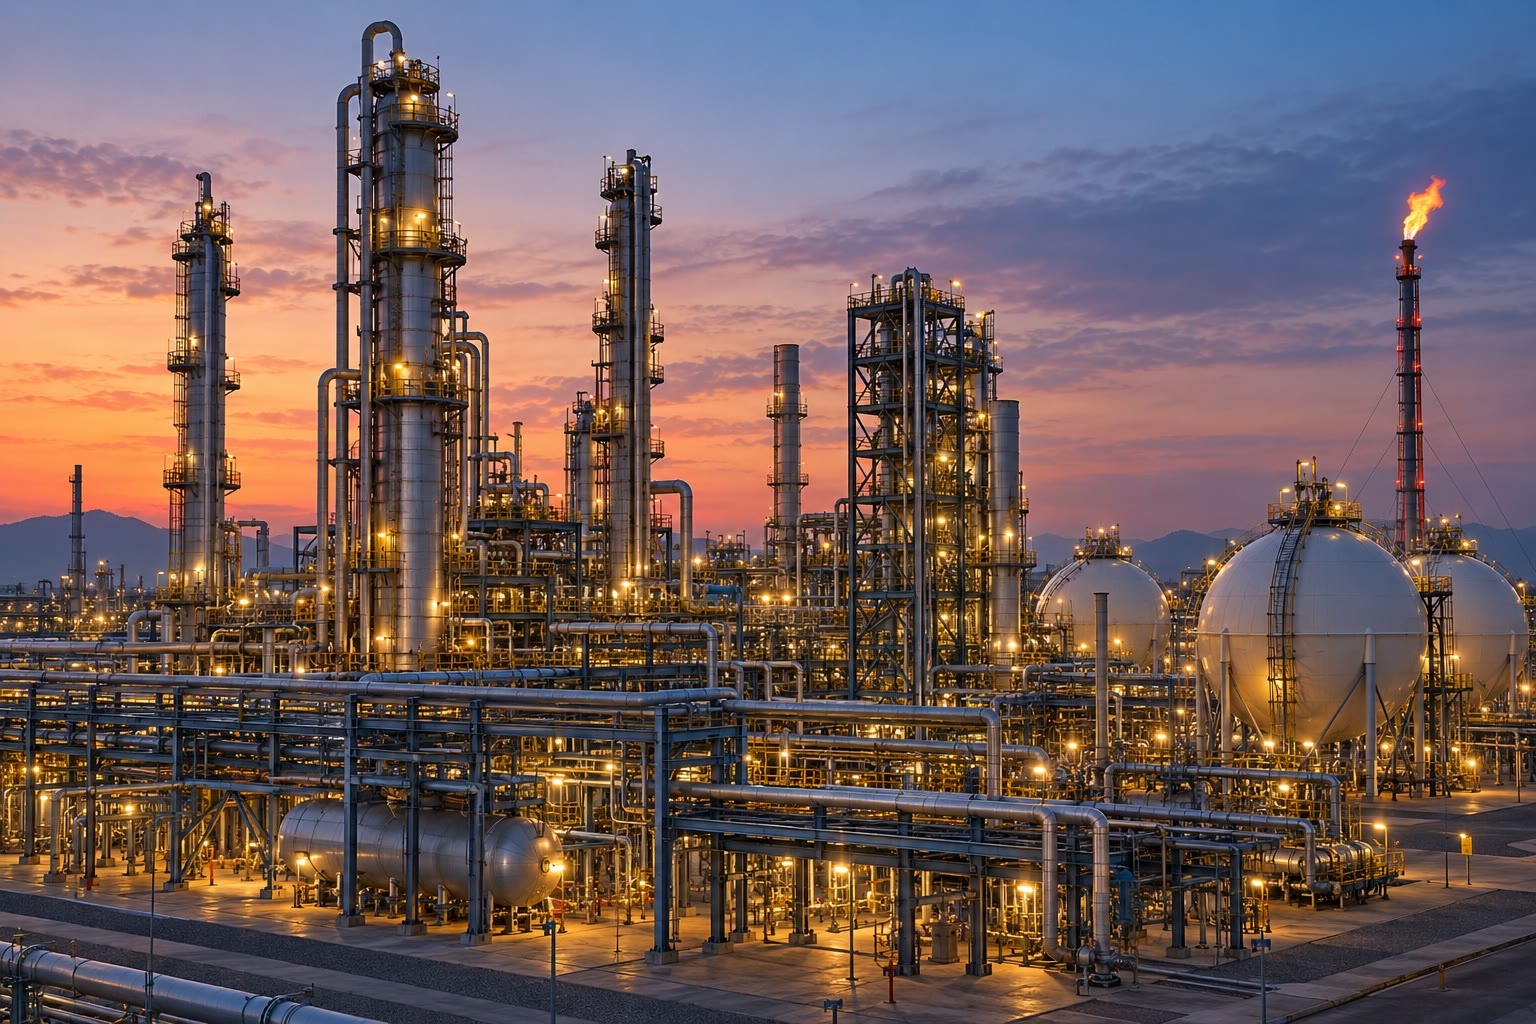
\includegraphics[width=0.6\linewidth]{images/book4/ai/b3-16-ammonia-plant.jpg}

{\small 一座合成氨装置。其核心反应器中装有数吨
添加助剂的铁催化剂；装置的大部分用于制备氢气，并
使未转化的气体循环利用。}
\end{omfigure}

\section{表面观测}

\begin{definition}[程序升温脱附]\label{def:b3:surfaces-catalysis:tpd}
\emph{程序升温脱附}\index{程序升温脱附}
是以恒定速率加热带有\omterm{def:b3:surfaces-catalysis:adsorption}{吸附质}的表面，并记录
\omterm{def:b3:surfaces-catalysis:adsorption}{脱附}出的气体（用质谱仪测定）；每一结合态给出一个峰，其
峰温随\omterm{def:b3:surfaces-catalysis:adsorption}{脱附}活化能的增大而升高。
\end{definition}

\omterm{def:b3:surfaces-catalysis:adsorption}{脱附}峰的位置给出\omterm{def:b3:surfaces-catalysis:adsorption}{脱附}能（对于一级\omterm{def:b3:surfaces-catalysis:adsorption}{脱附}，
$E_d \approx RT_{\mathrm p}[\ln(\nu T_{\mathrm p}/\beta) - 3.64]$，式中 $\beta$ 为升温速率，$\nu \approx \qty{e13}{s^{-1}}$，
在本阶段不加证明地承认），其面积给出\omterm{def:b3:surfaces-catalysis:adsorption}{吸附}量。以 X 射线为激发源的光电子能谱
（XPS）测量表面原子内层电子的结合能，
由此可确定表层前几纳米内的元素及其氧化态。
扫描隧道显微镜使一根尖锐的针尖在导电表面上方
零点几纳米处移动；隧道电流
（见\cref{ch:b3:quantum-model-systems}）在距离
每增加 \qty{0.1}{nm} 时约降低一个数量级，因此扫描时保持电流恒定，
即可逐个原子地描绘出表面。

\begin{inthelab}[BET 测量]
称取约 \qty{0.2}{g} 样品装入带灯泡的玻璃管，
在真空中于 150 至 \qty{300}{\celsius} 下脱气数小时，再次称重后安装到仪器上，
灯泡浸入液氮杜瓦瓶中。
分次通入少量氮气，每次通入后测量平衡压强，
由气体平衡求得\omterm{def:b3:surfaces-catalysis:adsorption}{吸附}量；玻璃管的死体积
用不\omterm{def:b3:surfaces-catalysis:adsorption}{吸附}的氦气测量。
\end{inthelab}

\begin{safety}{\ghs[0.7cm]{GHS06}\ghs[0.7cm]{GHS07}\ghs[0.7cm]{GHS08}\ghs[0.7cm]{GHS09}}
% ledger: ghs4:V2O5, ghs4:Ni
还原后的金属催化剂（负载于载体上的细粉状镍、钯或铂，
刚在氢气中还原）遇空气可能自燃：应在惰性气体中操作，
储存前需钝化处理。镍是皮肤致敏物，
也是疑似致癌物；五氧化二钒吸入或误食有毒，
并可能致癌。催化剂粉末应在
通风密闭装置中称量。
\end{safety}

\begin{history}[朗缪尔与氨催化剂]
欧文·朗缪尔在工业实验室研究灯泡时，
从\omterm{def:b3:surfaces-catalysis:adsorption}{吸附}气体形成\omterm{def:b3:surfaces-catalysis:coverage}{单分子层}的设想出发，于 1916 至 1918 年导出了他的等温式；
因表面化学方面的工作，于 1932 年获得诺贝尔化学奖。
数年前，阿尔温·米塔施曾组织寻找实用的氨催化剂：
在小型高压反应器中测试了数千种组成，
最终选定了至今仍在使用的助催化铁催化剂。
这是最早的系统性催化剂筛选之一。
\end{history}

\section{练习}

\begin{exercise}[$\star$]\label{exo:b3:surfaces-catalysis:1}
气体在 \qty{2.0}{kPa} 下覆盖了朗缪尔表面的 40\,\%。求 $K$ 以及
\qty{10}{kPa} 下的\omterm{def:b3:surfaces-catalysis:coverage}{覆盖度}。
\end{exercise}

\begin{exercise}[$\star$]\label{exo:b3:surfaces-catalysis:2}
在某金属上测得两个\omterm{def:b3:surfaces-catalysis:adsorption}{吸附}焓：$-20$ 和 \qty{-150}{kJ/mol}。
哪一个是\omterm{def:b3:surfaces-catalysis:physi-chemi}{物理吸附}，哪一个是\omterm{def:b3:surfaces-catalysis:physi-chemi}{化学吸附}？哪一个可能是解离\omterm{def:b3:surfaces-catalysis:adsorption}{吸附}？
\end{exercise}

\begin{exercise}[$\star$]\label{exo:b3:surfaces-catalysis:3}
对于面心立方金属的 (100) 面和
(111) 面，计算每个表面原子对应的顶位、桥位和穴位的数目。
\end{exercise}

\begin{exercise}[$\star$]\label{exo:b3:surfaces-catalysis:4}
某催化剂每克每秒转化 \qty{3.0e-6}{mol} 反应物，
每克含 \qty{1.5e-5}{mol} 表面\omterm{def:b3:complex-kinetics:enzyme}{活性位点}。求转化频率。
\end{exercise}

\begin{exercise}[$\star\star$]\label{exo:b3:surfaces-catalysis:5}
氢气以解离方式\omterm{def:b3:surfaces-catalysis:adsorption}{吸附}，在 \qty{1.0}{kPa} 下 $\theta = 0.10$。求 \qty{4.0}{kPa} 下的 $\theta$。
\end{exercise}

\begin{exercise}[$\star\star$]\label{exo:b3:surfaces-catalysis:6}
CO（$K = \qty{10}{kPa^{-1}}$）与 \ce{O2}（$K = \qty{0.5}{kPa^{-1}}$，在此简单模型中为非解离\omterm{def:b3:surfaces-catalysis:adsorption}{吸附}）
在 1.0 和 \qty{5.0}{kPa} 下竞争铂表面的\omterm{def:b3:surfaces-catalysis:adsorption}{吸附}位点。求两者的
\omterm{def:b3:surfaces-catalysis:coverage}{覆盖度}，并讨论 CO 氧化速率。
\end{exercise}

\begin{exercise}[$\star\star$]\label{exo:b3:surfaces-catalysis:7}
在 \qty{300}{K} 下于 \qty{1.0}{kPa} 达到的某一\omterm{def:b3:surfaces-catalysis:coverage}{覆盖度}，在 \qty{350}{K} 下需要 \qty{8.0}{kPa}。求\omterm{def:b3:surfaces-catalysis:isosteric}{等量
吸附焓}。
\end{exercise}

\begin{exercise}[$\star\star$]\label{exo:b3:surfaces-catalysis:8}
% ledger: sa:N2.am, const:Vm1, const:NA
某活性炭的 $v_{\mathrm m} = \qty{120}{cm^3.g^{-1}}$（标准状况，273.15 K 和
\qty{101.325}{kPa}）。求其 BET 面积。
\end{exercise}

\begin{exercise}[$\star\star$]\label{exo:b3:surfaces-catalysis:9}
铂上 $\ce{2 CO + O2 -> 2 CO2}$ 的反应速率随 $p(\ce{CO})$ 增大
（$p(\ce{O2})$ 固定）先升高、再经过极大值后下降。这说明采用何种机理？CO
为何会抑制反应？
\end{exercise}

\begin{exercise}[$\star\star\star$]\label{exo:b3:surfaces-catalysis:10}
某表面反应的真实活化能为 \qty{100}{kJ/mol}；反应物的
$\Delta_{\mathrm{ads}}H = \qty{-60}{kJ/mol}$。在低\omterm{def:b3:surfaces-catalysis:coverage}{覆盖度}和高\omterm{def:b3:surfaces-catalysis:coverage}{覆盖度}下分别测得的活化能是多少？
在较宽的温度范围内画出 $\ln r$ 对 $1/T$ 的示意图。
\end{exercise}

\begin{exercise}[$\star\star\star$]\label{exo:b3:surfaces-catalysis:11}
硫在镍催化剂上\omterm{def:b3:surfaces-catalysis:adsorption}{吸附}，\omterm{def:b3:surfaces-catalysis:coverage}{覆盖度}为 0.10（每个表面 Ni 原子上的硫原子数），
每个硫原子占据四个位点。对于只需一个空位点的反应，剩余活性占原来的几分之几？
对于需要两个相邻空位点的反应（假设
被占据位点随机分布）呢？
\end{exercise}

\begin{exercise}[$\star\star\star$]\label{exo:b3:surfaces-catalysis:12}
对于合成氨，三种金属结合原子态氮的焓分别为
$-150$、$-250$ 和 \qty{-400}{kJ/mol}（练习数据）。利用\omterm{def:b3:surfaces-catalysis:sabatier}{萨巴蒂尔
原理}，哪一种可能是最佳催化剂？另外两种受什么限制？
\end{exercise}

\section{问题：测量催化剂}

\begin{problem}[{周末问题——测量催化剂：负载铂催化剂的 BET 比表面积、
金属分散度和颗粒尺寸（由氢化学吸附测定），
以及氢化反应的转化频率}]
\label{pb:b3:surfaces-catalysis:1}
% ledger: sa:N2.am, lat:Pt, aw:Pt, const:Vm1, const:NA
某催化剂含 1.00\,\% 质量分数的铂，负载于氧化铝上。问题数据：
77\,K 下的氮气等温线（标准状况下的体积，273.15 K 和
\qty{101.325}{kPa}，每克）：
\begin{center}\small
\begin{tabular}{lcccccc}
\hline
$x = p/p^*$ & 0.05 & 0.10 & 0.15 & 0.20 & 0.25 & 0.30 \\
$v$ / \unit{cm^3.g^{-1}} & 41.2 & 46.1 & 51.1 & 54.1 & 58.9 & 62.9 \\ \hline
\end{tabular}
\end{center}
\ce{H2} \omterm{def:b3:surfaces-catalysis:physi-chemi}{化学吸附}于铂上：每克催化剂 \qty{0.205}{cm^3}。某氢化反应
在每克催化剂上以 \qty{2.0e-5}{mol} 每秒的速率进行。铂：$M = \qty{195.08}{g/mol}$，面心立方，
$a = \qty{392.3}{pm}$；标准状况下气体摩尔体积 \qty{22414}{cm^3/mol}；
$a_{\mathrm m}(\ce{N2}) = \qty{0.162}{nm^2}$。

\medskip\noindent\textbf{第一部分——BET 作图。}
\begin{enumerate}
  \item 为什么要在 \qty{77}{K} 下测量等温线？
  \item 为什么只用 0.05 到 0.30 之间的相对压强？
  \item 计算各数据点的 $x/(v(1 - x))$。
  \item 最小二乘直线的斜率为 \num{0.02205}，截距为 \num{0.000180}
        （单位为 \unit{g.cm^{-3}}）。由此求 $v_{\mathrm m}$。
  \item 求 $c$。较大的 $c$ 意味着什么？
  \item 为什么截距确定得如此不准？它对 $v_{\mathrm m}$ 的求值有影响吗？
\end{enumerate}

\medskip\noindent\textbf{第二部分——面积。}
\begin{enumerate}[resume]
  \item 计算每克样品\omterm{def:b3:surfaces-catalysis:coverage}{单分子层}中氮的物质的量。
  \item 计算\omterm{def:b3:surfaces-catalysis:surface-area}{比表面积}。
  \item 固体的哪一部分提供了几乎全部的这一表面积？
  \item 对于沸石等微孔固体，BET 方法为什么会失效？
\end{enumerate}

\medskip\noindent\textbf{第三部分——分散度与粒径。}
\begin{enumerate}[resume]
  \item 计算每克催化剂上\omterm{def:b3:surfaces-catalysis:physi-chemi}{化学吸附}的 H 原子的物质的量。
  \item 计算每克催化剂中铂的物质的量。
  \item 由此求分散度。
  \item 计算体相中每个 Pt 原子的体积。
  \item 对 (111)、(100) 和 (110) \omterm{def:b3:x-ray-diffraction:miller}{晶面}取平均后，每个表面原子的面积为
        \qty{0.0807}{nm^2}。请核对 (111) 面的值 $\frac{\sqrt3}{4}a^2$。
  \item 证明对球形粒子有 $d = 6v_{\mathrm{at}}/(a_{\mathrm{at}}D)$。
  \item 计算平均粒径。
  \item 哪些假设限制了这一结果的适用范围？
\end{enumerate}

\medskip\noindent\textbf{第四部分——催化活性。}
\begin{enumerate}[resume]
  \item 计算每个表面 Pt 原子的转化频率。
  \item 计算每克铂的反应速率。
  \item 若颗粒在转化频率不变的条件下\omterm{def:b3:surfaces-catalysis:catalyst-design}{烧结}至 \qty{10}{nm}，每克的反应速率将
        下降多少倍？
  \item 若转化频率随粒径而变化，这说明了什么？
  \item 为什么比较催化剂时用转化频率，而不用
        每克的反应速率？
  \item 给出结果：铂颗粒的平均直径。
\end{enumerate}
\end{problem}
